\documentclass[../Relazione.tex]{subfiles}

\begin{document}

\section{Il contenuto e la navigabilità}

	\subsection{Il testo}
		Data la tipologia informativa e commerciale del sito internet non è richiesto che il testo abbia tante accortezze linguistiche come, per esempio, un sito giornalistico. Si è quindi analizzato che il testo rispettasse le regole base di usabilità:
		\begin{itemize}
			\item \textbf{Dimensione} del testo adatta e \textbf{leggibilità};
			\item Supporto dell'opzione \textbf{zoom} del browser;
			\item Tipologia di \textbf{font};
			\item \textbf{Contrasto} tra testo e sfondo;
			\item Presenza di una \textbf{Struttura} del testo;
		\end{itemize}
		
		\subsubsection{Dimensione e leggibilità}
			La dimensione del testo è impostata su 14pt nella \emph{Homepage} e 12pt nella pagina \emph{Contatti}, quindi superano entrambi quella minima consigliata (10pt). Molto grave la dimensione del testo troppo piccola (9pt) nella pagina \textbf{''Dove siamo''} che dovrebbe spiegare con chiarezza dove si trova la struttura. Ancora peggiore è la dimensione font ad 8 pt nella pagina \textbf{''Listino''}: praticamente solo le parole colorate in rosso sono abbastanza leggibili e percepili come informazioni, ma ancora troppo piccole. Inoltre le scritte sono raggruppate e contornate da un bordo rosso che rende il tutto quasi illeggibile senza uno zoom.
			Il testo in grassetto con font maggiore è ben posizionato. Viene utilizzato per alcune keyword nella \emph{Homepage}, per i nomi delle sezioni nel menu orizzontale e in alcune parti di altre pagine la scrittura in stampatello maiuscolo e questo, se pur poco, diminuisce l'usabilità dell'utenza abituata a leggere in stampatello minuscolo.
			Molto insufficiente questa parte riguardante il testo.
			
		\subsubsection{Zoom}
			Il sito non presenta un'opzione di zoom interna. Si è quindi provato ad utilizzare lo zoom implementato nel browser per analizzare se questo fosse supportato, ossia se la pagina degradasse elegantemente e mantenesse la leggibilità del testo. 
			La funzionalità zoom è permessa e nei maggiori browser (IE, Safari, Chrome, Firefox) funziona perfettamente, la leggibilità permane abbastanza nei contenuti testuali grazie al layout del sito responsive.
			Anche la funzionalità di aumento della dimensione dei caratteri interna al browser funziona bene.
			Punto negativo: ad un certo punto se si ingrandisce troppo il sito passa alla modalità mobile.
			Punto a favore: non si presente mai la barra orizzontale per lo scroll ma il testo si adatta sempre.
	
		\subsubsection{Font}
			La tipologia del font è personalizzata, l'ordine dei font è {\textbf{tahoma}, arial, helvetica, sans-serif;}
			Il font Verdana, quello più apprezzato secondo gli utenti, non è impostato e nemmeno tra le scelte alternative.
			
		\subsubsection{Contrasto}
		\begin{itemize}
            \item \textbf{Corpo}
            \vspace*{5mm}\\Nella pagine \textbf{Eventi} in quella \textbf{Listino} lo sfondo sotto al testo è di colore bianco, per cui perfettamente leggibile anche se il colore del testo per le keyword a volte è rosso.
			Sempre nella pagina \emph{Listino} Il testo sovrapposto alle immagini risulta sempre visibile grazie all'utilizzo di coppie di colori ben distinguibili tra loro mantenendo quindi un buon contrasto ed una corretta comprensibilità.
			Nelle altre pagine lo sfondo sotto al testo non è del tutto bianco, ma presenta una leggera trasparenza che lascia intravedere l'intera immagine di background applicata come sfondo base del sito web.\\
			Nonostante ciò il contrasto tra testo e sfondo non è compromessa e le informazioni rimangono ben leggibili in quanto il testo presente è sempre di colore nero/blu molto scuro.\\
			\item \textbf{Menù di navigazione}
            \vspace*{5mm}\\Infine il testo applicato nel menù di navigazione: Esso è chiaramente visibile e ben distinguibile per colori e contrasto, il testo è bianco, con font maiuscolo e grassetto, contornato da uno sfondo mimetico rosso per evidenziare in che pagina ci troviamo, nelle altre pagine il testo tende leggermente verso il grigio, come si vede dall'esempio sottostante.

            	\begin{figure}[!h]
            		\centering
            		
\includegraphics[scale=0.7]{img/contenuto/Testo.png}
            		\caption{Testo - contrasto colori nel menù di navigazione orizzontale}
            		\label{fig:label}
            	\end{figure}

        \end{itemize}
			
			
		\subsubsection{Struttura}
			Il testo è sempre suddiviso in blocchi ben distinti con un titoletto iniziale e durante l'analisi non si sono mai trovati muri di testo. Questo garantisce maggior leggibilità e incoraggia l'utente alla lettura. Nella \textbf{Homepage} le 3 immagini statiche sotto il menù impediscono all'utente di leggere le informazioni sottostanti, che risultano tagliate.
			In tal caso un rimedio potrebbe essere di ridurre sostanzialmente la dimensione delle immagini, di affiancarle al testo, di spostarle al di sotto o addirittura di eliminarle viste la presenza di una pagina \textbf{Gallery} tutta dedicata a questo scopo.
						
	
	\newpage
	\subsection{Le immagini}\label{sec:img}
		Il sito presenta una grossa attenzione alle immagini, posizionandole talvolta come se fossero di priorità maggiore rispetto al testo.
		Come già fatto presente, sono presenti pagine che basano tutto il contenuto informativo (testuale) tramite immagini contenenti testo.
		Questa logica è da evitare in modo assoluto in quanto un interruzione del loro caricamento lascerebbe spoglia tale pagina da informazioni. (riferimento: Figura \textbf{\ref{fig:noInfo}})\\\\
		Dalla figura della \textbf{Homepage} (Figura \textbf{\ref{fig:homepage}}) inoltre, si può  intuire quanto lo \textbf{scroll} aggiuntivo sia causato dallo spazio occupato dalle immagini soprastanti il testo. Il numero di parole all'interno nella pagina infatti è tale da poter essere incluso totalmente nella prima schermata eliminando quasi del tutto l'utilizzo dello scroll.\\
		Inoltre un altro grave riscontro sta nella non ``cliccabilità'' di alcune immagini! Prendendo sempre la homepage come riferimento, si evince che solo le immagini associate ai link esterni dei social networks e quelle degli sponsor nel footer sono cliccabili, altre foto come quelle che ''rompono'' il contenuto informativo sono statiche.\\\\
		Le immagini hanno un tasso di click superiore al testo, solitamente il 20\% degli utenti clicca sull'immagine. Per sfruttare questo, tutte le immagini dovrebbero essere cliccabili con evento correlato, l’utente è statisticamente abituato a cliccarci sopra e si aspetta sempre qualcosa.
		In conclusione, un'enorme quantità di immagini, anche non cliccabili, con più importanza rispetto al testo. La maggioranza di esse non rappresentano link ipertestuali (click a vuoto dell'utente), ma vero e proprio contenuto informativo.

	\subsection{Breadcrump}
		Come già anticipato il tipo di breadcrump utilizzato è quello ad \textbf{attributi}. Ogni pagina del sito ha infatti infatti associato un tag con la tematica che tratta.
		Nonostante questo sia molto utile per comprendere subito l'argomento ed adatto alla gerarchia semplice del sito, non soddisfa pienamente i canoni di usabilità.
		Infatti si può notare dall'immagine sotto, come il titolo della pagina non dia alcun riferimento di che sito si tratti.\\ \textbf{Viene riportato solamente l'attributo di argomento.}\\
		La soluzione sarebbe ovviamente di inserire come minimo il nome del sito in cui l'utente sta navigando.

		\begin{figure}[!h]
			\centering
			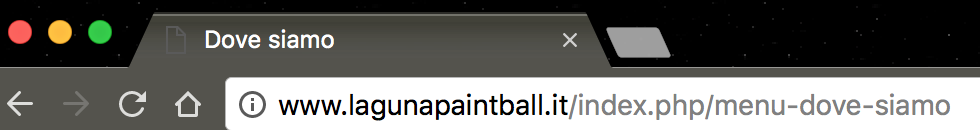
\includegraphics[scale=0.7]{img/contenuto/bread.png}
			\caption{Attribute Breadcrumb - Nella scheda appare solo il tag e non il nome del sito (Chrome v58)}
			\label{fig:label}
		\end{figure}
		
\newpage
	\subsection{Il footer}
		Una nota a parte va fatta per la componente del footer, che viene ripetuta in quasi tutte le pagine del sito, a meno della pagina \textbf{Gallery}.\\
		Esso è composto da due parti:
		\begin{itemize}
			\item Parte superiore: immagini;
			\item Parte inferiore: testo.
		\end{itemize}
		\underline{Nella parte superiore} son presenti 3 piccole immagini linkate ai social networks esterni al sito, esattamente come nell'header, nella parte centrale. A destra invece, sono presenti altre 3 immagini, di scarsissima qualità e risoluzione, anch'esse linkate a fonti esterne.
		Più nel dettaglio, le prime due sono dei link a dei siti web di affiliazione ed informazione, mentre la terza genera un invio mail ad un indirizzo personalizzato.
		Questa differenza non è assolutamente evidente, genera disorientamento per l'utente e provoca \emph{Gambling click}, poichè l'utente crede di generare la stessa azione per 3 immagini che sono ordinate e presentate in modo equivalente. \\\\
		\underline{Nella parte inferiore} è presente del testo, centrato sia come riferimento spaziale nel footer che come orientamento.\\
		Il testo è formato a sua volta da 3 righe: la prima e l'ultima con colorazione sul blu scuro, mentre quella di mezzo nera. Seppur minima questa differente colorazione è evidente.\\
		Queste informazioni contengono riferimenti a copyright, indirizzo di sede sociale e di design del sito, come è giusto siano contenute nel footer.
		Il problema in questa parte risiede in altro: le colorazioni diverse del testo non anticipano alcuna differenza funzionale, si tratta infatti sempre di testo statico; nessun link.
		L'utente è perciò confuso dalla diversa colorazione sopra e sotto che fa credere a dei link generando ancora una volta \textbf{gambling click} e \textbf{metafore visive}.

		\begin{figure}[!h]
			\centering
			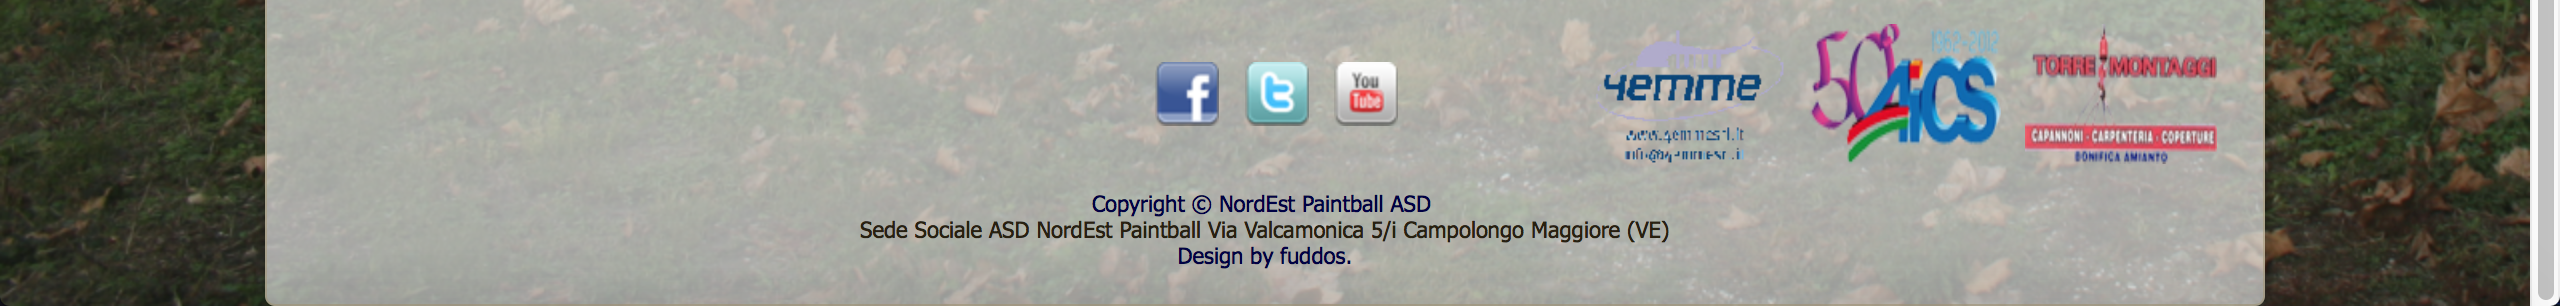
\includegraphics[width=0.7\textwidth]{img/contenuto/Footer.png}
			\caption{il \textbf{Footer} del sito - Si può notare come non esista divisione grafica dal body}
			\label{fig:label}
		\end{figure}
		
	\subsection{Metafore visive}
		Riassumiamo per chiarezza le metafore visive nel sito.\\
		Per metafora visiva si intende l'uso di effetti grafici che ingannano l'aspettativa dell'utente. Nel sito sono presenti varie metafore visive.
		\subsubsection{Pagine già analizzate}
		Prima fra tutti quella delle \textbf{immagini non riconosciute come immagini} già precedentemente notata e più volte rimarcata.\\\\			
		Nella homepage solamente le icone nell'header e nel footer sono cliccabili e conducono l'utente altrove, tutte le altre sono finti link.\\\\			
		La seconda metafora visiva la troviamo nei \textbf{finti link} di colorazione blu scuro del footer.\\L'utente non ha modo all'interno del sito di capire se un testo è un link e risulta difficile se non impossibile la comprensione di tale stile applicato in modo differente su elementi uguali.
		\subsubsection{Gallery - Pagina interna}
		La terza ed ultima metafora visiva la troviamo all'interno della pagina \textbf{Gallery}, non analizzata a livello d'usabilità poichè composta, quasi nel completo, solo da uno slider di immagini (pure di scarsa qualtà).\\
		Escluso l'errore banale di mettere una slideshow automatica, che per l'utente crea disagio e confusione non controllata, la metafora visiva si presenta proprio in questa sequenza di immagini, capiamo meglio come.\\
		Come possiamo vedere dall'immagine poco sotto, la slideshow è composta da una mini-sequenza di anteprima immagini, che sono selezionabili in base a quella che si vuole visualizzare ed il riquadro soprastante dove è visualizzata l'immagine vera e propria.
		Entrambi queste componenti sono cliccabili e scatenano un evento, infatti l'hover del mouse suggerisce che si tratta di questo. Il problema è che l'icona del mouse è uguale in entrambe le parti ma le azioni che ne conseguono al click sono differenti:
		\begin{itemize}
			\item \textbf{Per gli anteprima:} la conseguenza al click cambia l'immagine visualizzata sopra in grande;
			\item \textbf{Per le immagini in preview:} la conseguenza al click mostra la stessa immagine ma in un riquadro più piccolo (dove è possibile continuare a vedere le successive) e scurendo il background.
		\end{itemize}
		Si può quindi capire come l'utente sia decisamente disorientato e costretto a fare operazioni inutili per tornare indietro, visto il nessun vantaggio ricevuto dal click all'immagine in grande.\\\\
		Come se non bastasse, sempre nella preview in grande, nell'angolo in basso a destra è presente una piccola icona (molto poco visibile!) che simboleggia un ingrandimento (vedi angolo suggerito, dalla figura: \textbf{\ref{fig:gallery}}).\\
		Tale icona viene illuminata al passaggio del puntatore ma l'icona dell'hover non cambia.\\
		\underline{Cosa succederà mai se un utente ci clicca sopra?}\\
		Propio una bella domanda, visto che il click causerà un'\textbf{azione del tutto differente} dalle 2 precedenti: lo slideshow (e quindi l'immagine) ed il browser stesso si impostano in modalità ''a tutto schermo'' mantenendo la grafica e tutti i collegamenti descritti prima !!!\\
		L'icona nell'angolo basso a destra ora inverte le frecce ma al passaggio del mouse si illumina, ma ritorna con le frecce iniziali: dettaglio estremamente fuorviante per l'utente.
		Concludendo il discorso, tutto ciò crea una incontrollata ed inaspettata sorpresa/perplessità da parte dell'utente, soprattutto riguardo i legami logici tra icone --> conseguenza all'interno di questo sito.\\
		Costruzione del tutto insensata per questa componente di preview immagini.
			
\newpage
		\begin{figure}[!h]
			\centering
			\includegraphics[width=\textwidth]{img/contenuto/gallery.png}
			\caption{Pagina \textbf{Gallery} - Metafora visiva creata dalla slideshow (Chrome v58) - (\url{http://www.lagunapaintball.it/index.php/menu-gallery})}
			\label{fig:gallery}
		\end{figure}

		\begin{figure}[!h]
			\centering
			\includegraphics[width=\textwidth]{img/contenuto/galleryClick.png}
			\caption{Pagina \textbf{Gallery} - Vista dopo un click su di una immagina in preview (Chrome v58)}
			\label{fig:galleryClick}
		\end{figure}

\newpage
	\subsection{Pagina 404}
		Può succedere di dover rimuovere delle pagine dal proprio o sito o semplicemente di doverle trasferire su un altra URL. È importante in questi casi pianificare come gestire eventuali errori 404 generati dagli utenti che magari fanno ancora riferimento alle pagine rimosse o spostate. Nel caso di pagine spostate l’approccio corretto è quello di utilizzare dei redirect, mentre per gli URL che non esistono più è buona pratica adottare una pagina apposita che informi l’utente e lo aiuti a proseguire la navigazione.\\\\
		In ogni caso una pagina 404 efficace spingerà l’utente a rimanere sul sito invece di uscire. L’utente deve accorgersi di essere arrivato su una pagina di errore, ma leggere la sola frase \emph{“Pagina non trovata”} accompagnata da un freddo \emph{“errore 404”} lo spingerà certamente ad uscire e cercare altrove ciò gli interessa.\\
		Quindi una pagina 404 deve catturare l’attenzione dell’utente e fornirgli degli strumenti per continuare la sua navigazione all'interno del sito.\\\\
		Detto ciò, \paint\ usa in maniera quasi del tutto corretta questo strumento di gestione dell'errore.
		Nel caso si voglia accedere ad una pagina nel sito il cui indirizzo non esiste, si viene portati ad una \textbf{pagina 404} bianca, contentente tale riquadro:

			\begin{figure}[!h]
				\centering
				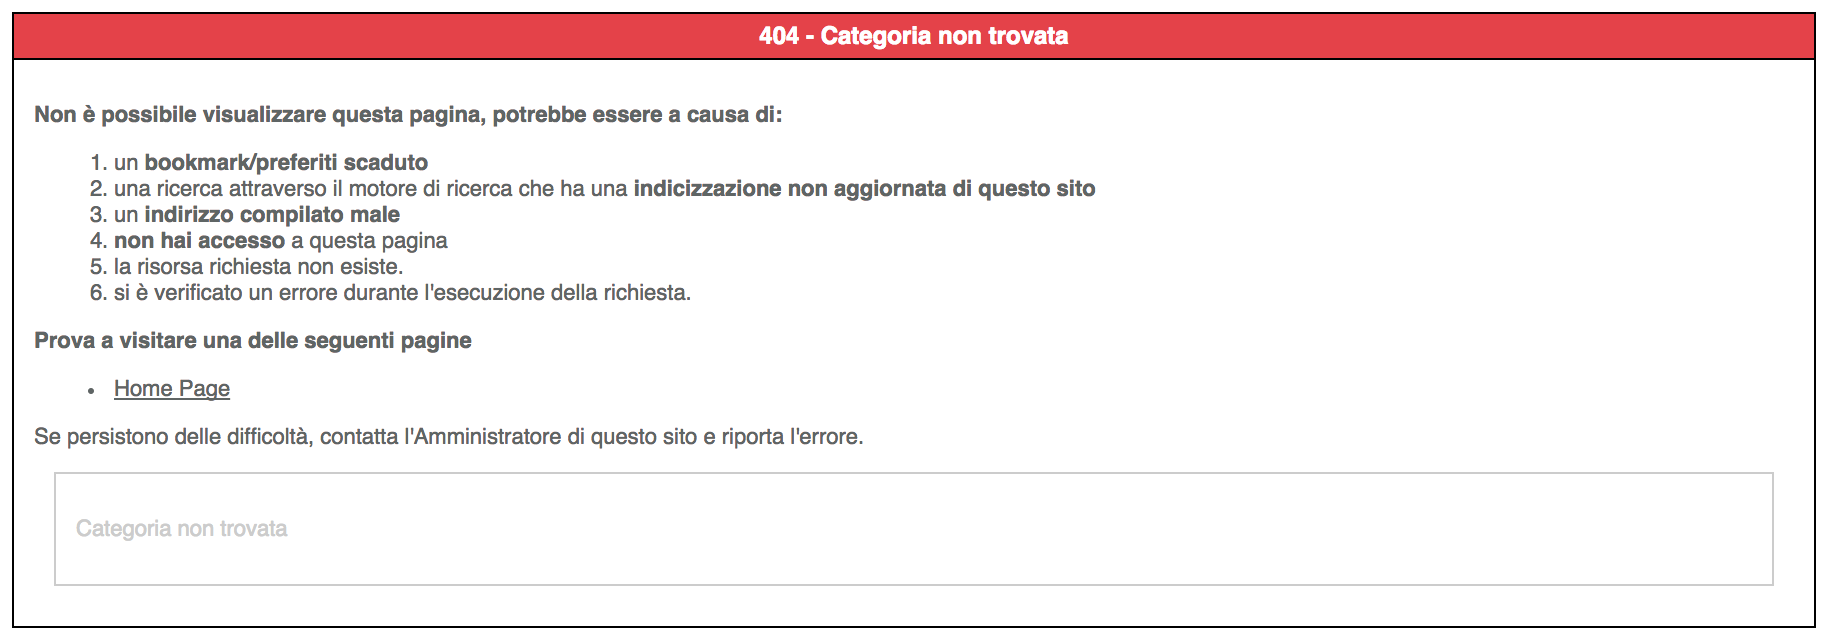
\includegraphics[width=0.90\textwidth]{img/contenuto/404.png}
				\caption{Gestione indirizzo mancante o inesistente - Pagina 404 (Chrome v58)}
				\label{fig:label}
			\end{figure}

		La finestra presenta in titolo l'avviso \textbf{''404 - Categoria non trovata''} scritto in rosso e quindi ben visibile.
		La scritta indica un errore specifico e non generico, perciò molto impreciso e disorientante per l'utente.
		Il testo informativo fornisce però una lista di possibili cause alla visualizzazione di questa pagina perciò l'utente sa che errore può aver commesso o quale ne è la causa.
		Viene fornito inoltre un link per tornare alla \emph{Homepage} e favorire l'orientamento all'utente.
		Ultimo fattore, purtroppo negativo, è la presenza di una \emph{textfield} per contattare l'amministratore del sito in caso di persistenza d'errore.
		Il problema è che, oltre all'assenza di un bottone per il \emph{submit} della segnalazione, quest'ultima non può nemmeno essere scritta poichè il \emph{textfield} presente è inattivo e presenta solamente un placeholder con suscritto ''Categoria non trovata''; in poche parole l'ultima parte informativa è totalente inutile e anzi, danneggia l'utente ed è per lui fonte di perdita di tempo.

\end{document}